\documentclass[onecolumn,aps, pre,amsmath,amssymb,longbibliography,12pt]{revtex4-2}
\usepackage{graphicx}
% \usepackage{dcolumn}
\usepackage{bm}
\usepackage{amsfonts}
\usepackage{xcolor,tabu}
\usepackage{multirow}
\usepackage{amsthm}
\usepackage{textcomp}
\usepackage{tikz}
\usepackage[colorlinks=true,
            linkcolor=blue,
            urlcolor=blue,
            citecolor=blue]{hyperref}
\hypersetup{bookmarksopen=true}
\usepackage{xr}
\usepackage{float}

\begin{document}
\title{Drop size control}
\maketitle

How the sizes of droplets influence the dynamics of the system, in particular the effective temperature of the active bath and the diffusivity of the inner droplet, is an important question in this project.
Using the capillary microfluidic device, we are able to vary continuously and seamlessly the flow rates of each phase to achieve precise control of drop sizes.
However, it is challenging to control the size of one droplet (inner/outer) independently, because each flow rate affects the sizes of both droplets.
As you can see in Fig.~\ref{fig:vary-middle}, when keeping both inner and outer flow rates constant and only varying the middle phase flow rate $Q_m$, the sizes of both droplets change.
It is most evident when contrasting the cases where $Q_m=700$ $\mu$l/h and $Q_m=200$ $\mu$l/h, where the shell shrinks as desired, but the inner droplet gets larger undesirably.

\begin{figure}[h]
  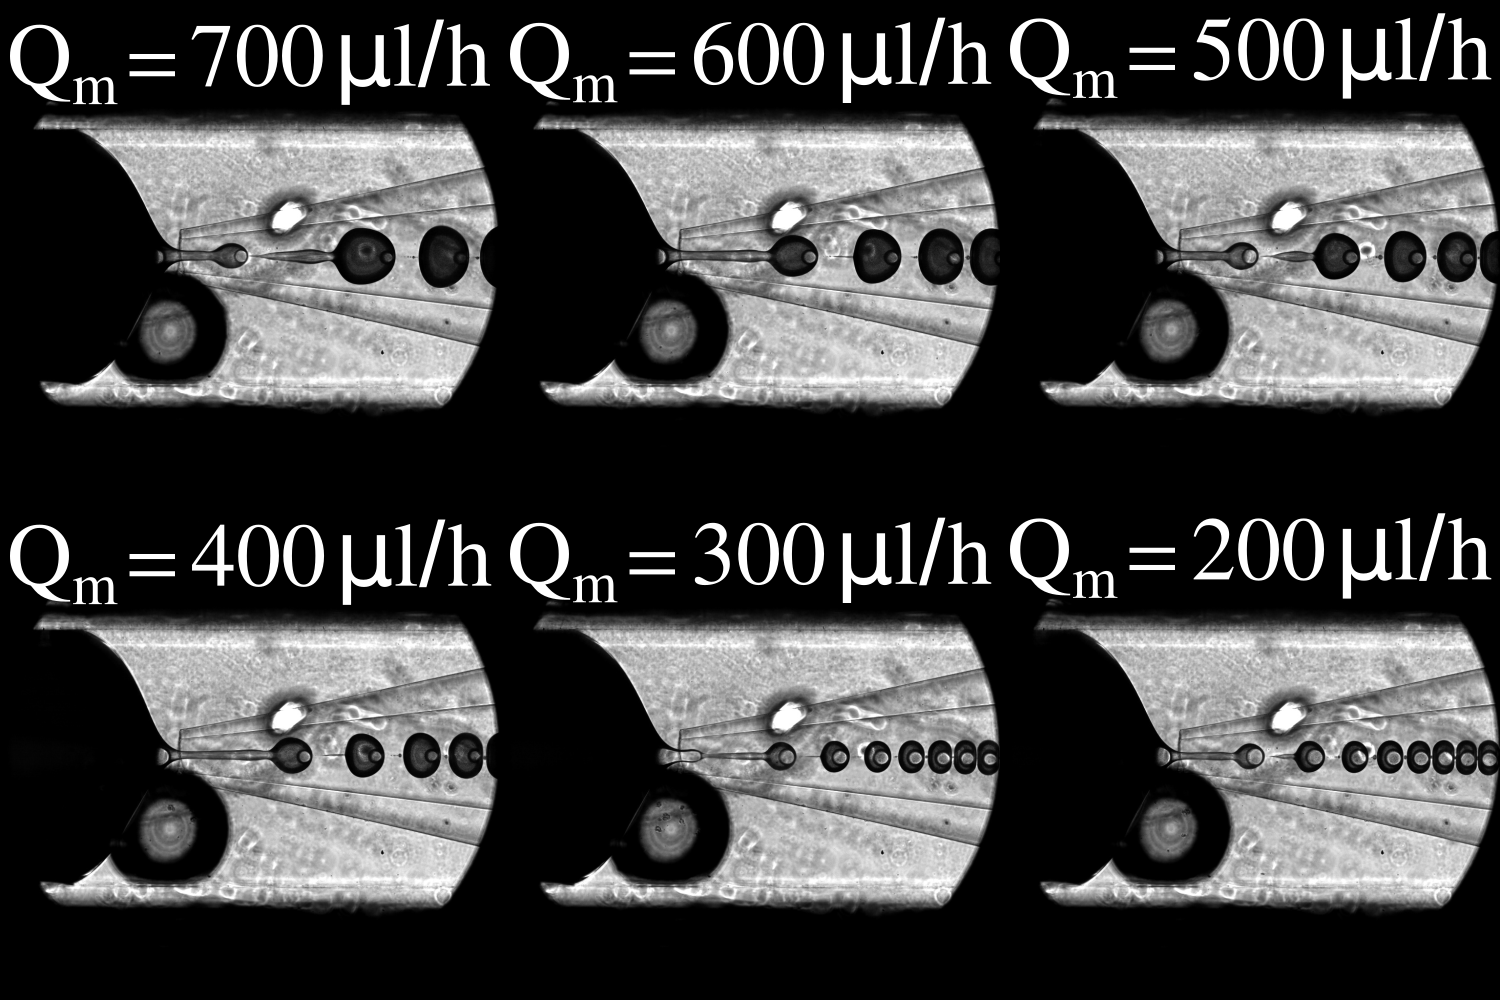
\includegraphics[width=5in]{vary-middle.png}
  \caption{Vary middle phase (bacterial suspension) flow rate $Q_m$ from 700 to 200 $\mu$l/h, while keeping outer and inner phase flow rates constant at $Q_o=1500$ $\mu$l/h and $Q_i=42$ $\mu$l/h.}
  \label{fig:vary-middle}
\end{figure}

The results in Utada et al. \cite{Utada2005} explains part of my observation.
Their results suggest that when fixing the sum of the middle and inner phase flow rates, as well as the ratio between the two, the sizes of both droplets only depend on the outer flow rate.
Figure \ref{fig:size-outerflow} illustrates the results of Utada et al., where $R$ is the size of droplets, $Q_o$ is the outer phase flow rate and $Q_{sum}=Q_i+Q_m$ is the sum of the inner and middle flow rates.
As a hypothesis, if we keep $Q_{sum}$ constant and vary the ratio between $Q_i$ and $Q_m$, we can keep the outer droplet constant size and explore the influence of the inner droplet size. A similar idea is that, if we keep $Q_o+Q_m$ and $Q_i$ constant, and vary the ratio between $Q_o$ and $Q_m$, the inner droplet size might be kept constant.

\begin{figure}[h]
  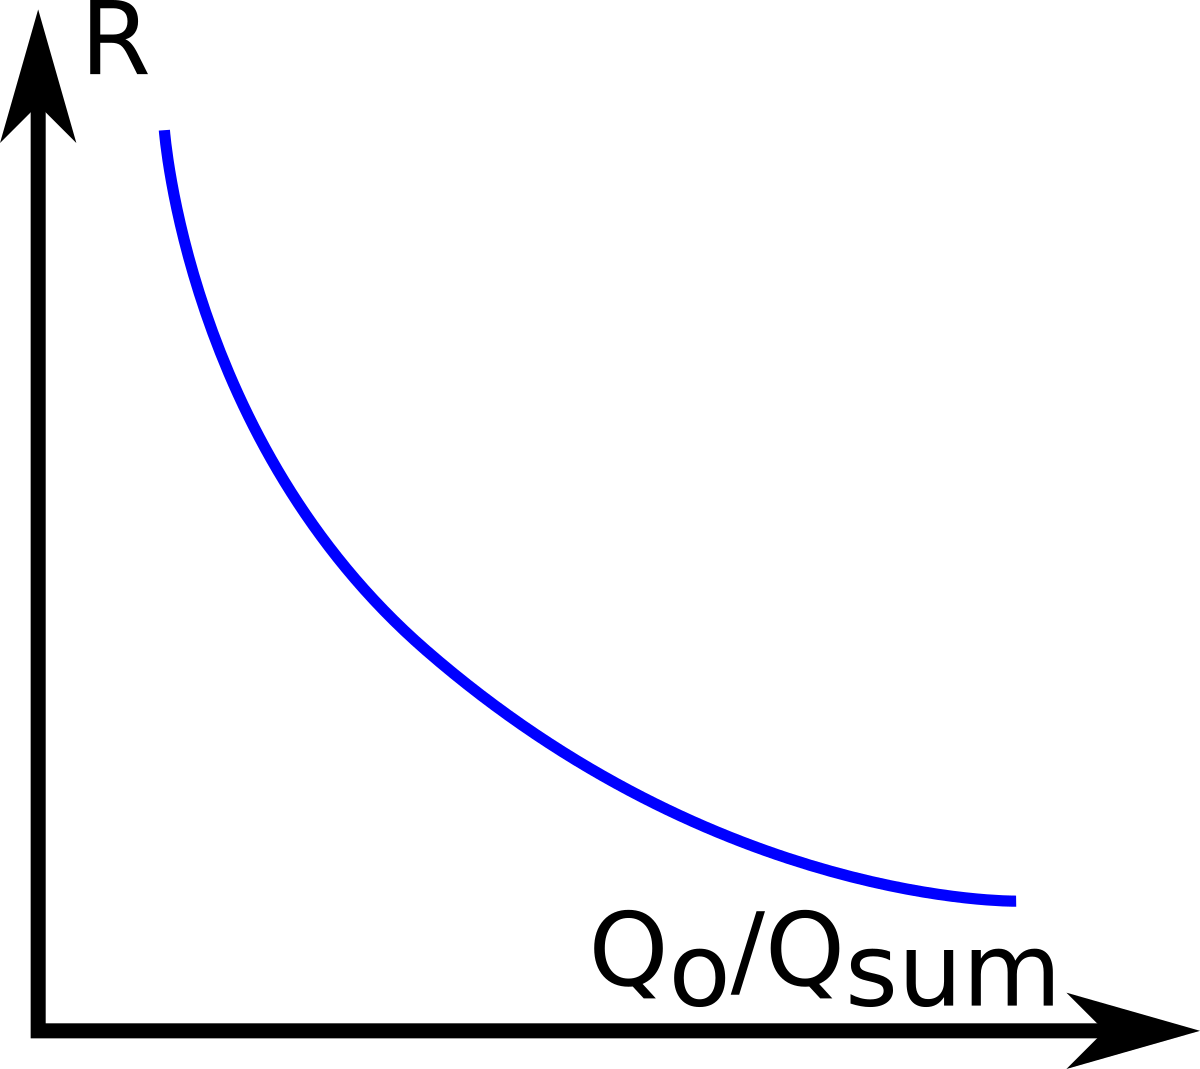
\includegraphics[width=3in]{size-outerflow.png}
  \caption{Double emulsion radius $R$ (only the outer droplet) depends on the ratio between outer phase flow rate $Q_o$ and the sum of inner and middle phase flow rates $Q_{sum}$.
  This is reproduced from Fig.~3 in \cite{Utada2005}.}
  \label{fig:size-outerflow}
\end{figure}

These two hypotheses remain are tested in my experiment (07132021).
First, I fixed the sum of middle and inner flow rates at $Q_m+Q_i=400$ $\mu$l/h.
The outer flow rate was also fixed, at $Q_o=1000$ $\mu$l/h.
During the test, I varied the ratio between $Q_m$ and $Q_i$ from 0.6 to 7.
And I expected that the inner droplet radii $r$ to decrease with increasing ratio, while the outer droplet radii $R$ remain unchanged.
Figure~\ref{fig:fix-mi-sum} shows the droplet sizes as a function of flow rate ratio $Q_m/Q_i$.
The empty markers denote the outer droplet radii $R$ and the solid markers denote the inner droplet radii $r$.
As I increase the ratio between $Q_m$ and $Q_i$, $r$ decreases as expected.
However, $R$ increases with $Q_m/Q_i$, contradicting my hypothesis.

\begin{figure}[h]
  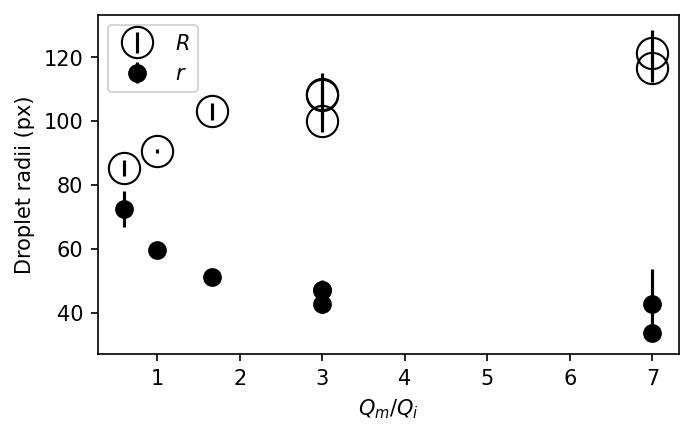
\includegraphics{fix-mi-sum.png}
  \caption{Double emulsion sizes as a function of the ratio between $Q_m$ and $Q_i$.
  The outer flow rate $Q_o$ and the sum of middle and inner flow rates are kept constant.}
  \label{fig:fix-mi-sum}
\end{figure}

Similarly, I fixed the sum of outer and middle flow rates at $Q_o+Q_m=1700$ $\mu$l/h.
The inner flow rate was also fixed, at $Q_i=100$ $\mu$l/h.
$Q_o/Q_m$ was varied from 3.25 to 7.5.
It is hypothesized that the inner droplet size remains constant, while the outer droplet size decreases with increasing $Q_o/Q_m$.
Figure~\ref{fig:fix-om-sum} shows the droplet sizes as a function of flow rate ratio $Q_o/Q_m$.
As I increase $Q_o/Q_m$, $r$ remains constant (approximately) while $R$ decreases, in consistency with my hypothesis.

\begin{figure}[h]
  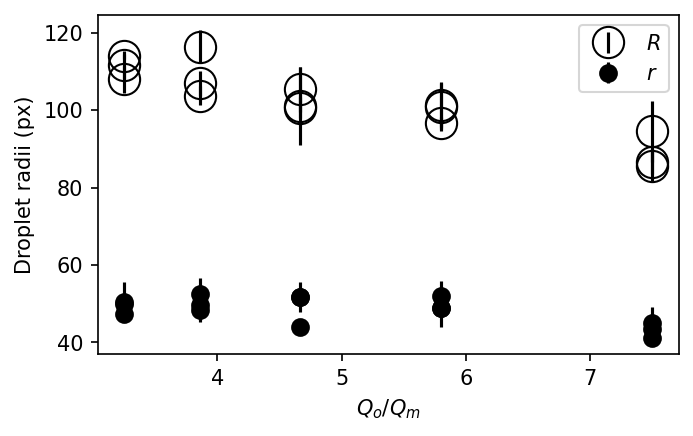
\includegraphics{fix-om-sum.png}
  \caption{Double emulsion sizes as a function of the ratio between $Q_o$ and $Q_m$.
  The inner flow rate $Q_i$ and the sum of outer and middle flow rates are kept constant.}
  \label{fig:fix-om-sum}
\end{figure}

\textcolor{red}{Why constant $Q_m+Q_i$ does not make outer droplet size constant?}

\bibliographystyle{apsrev4-2}
\bibliography{ref}

\end{document}
